% Sample file on how to use subfiles.
\documentclass[micro_gen.tex]{subfiles}

\begin{document}

\chapter{Microstructure generation}

In order to conduct numerical analyses of materials with a polycrystalline structure the geometrical properties of the grains in the material must be modeled. Interesting properties are the distribution of grain sizes, geometrical shape of the grains and orientation of the crystal lattices in the grains.

One possibility is to to extract the three dimensional microstructure from experiments in which for example X-ray microtomography is used. The images generated from such an experiment can be analyzed resulting in a digital representation of the microstructure, see for example \cite{Bhandari200722}. This is however a complicated process. The experiments required are extensive and expensive. When conducting multiscale modelling it would be desirable to be able to generate a large batch of different microstructures. This is so that variance in the results from the analyses with different microstructures can be studied to see if the model is large enough to represent a RVE. 
One would want a mathematically analytic description of a microstructure that is similar enough to the real structure of the material such that meaningful analysis can be done. One common way to do this is with the Voronoi tesselation. A Voronoi tessellation is a partition of a domain $D \in \mathbb{R}^d$ into $n$ regions $R_i$ in $D$, each corresponding to one of $n$ different \textit{seed points} $\vec{P}_i$. These regions consists of the set of all points that are closer to a particular seed point than to any other,
%
\[R_i = \{ \vec{x} \in D : \left|\left| \vec{P}_i - \vec{x} \right|\right| < \left|\left| \vec{P}_j - \vec{x} \right|\right| \quad  \forall i \neq j, \quad i,j = 1, \ldots, n \}. \]
%
In this thesis the norm used is the Euclidean distance, the dimension of the space is 3 and the bounding domain is a cube. In this case, the resulting regions will have the shape of convex polyhedrons which is referred to as \textit{grains}. This is the grain structure that would exist in a material where the grains started to nucleate at the seed points and all grew isotropically at the same rate. In a Voronoi tesselation two grains will intersect over a plane called a \textit{face},
three along a line called an \textit{edge} and four will intersect in a point called a \textit{vertex}. A common way to set the locations of the seed points is to randomly assign them to different positions in $D$. 
This is known as a "Poisson-Voronoi tesselation". An example of such a tessellation can be seen in figure \ref{fig:pois_voronoi} where 100 seed points have been used. The generation of the tessellation can easily be done in for example the commonly used software MATLAB \cite{matlab:voronoi}. In this thesis the open source software Neper \cite{Quey20111729} was used to generate the tessellation since this software is also capable of meshing the generated structure. 


Say that it represents the grains if grains would stelna uniform rate

Examples where Voronoi has been used

It is also possible to generate a periodic Voronoi tesselation. The method of doing this is by 
26 copies

This is done by duplicating the box containing the seed points 

\cite{Fritzen2009}



\begin{figure}
\centering
\begin{subfigure}[b]{.5\textwidth}
  \centering
  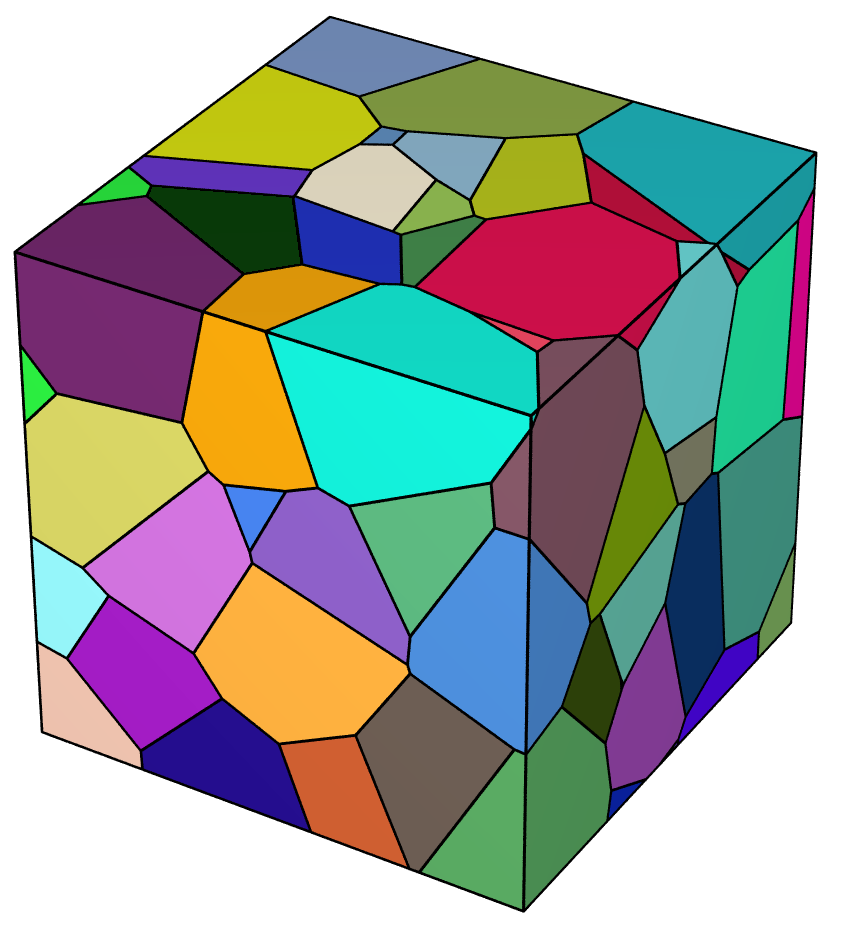
\includegraphics[width=.5\linewidth]{./figures/img_body.png}
  \caption{All polyhedrons shown.}
  \label{fig:pois_voronoi_a}
\end{subfigure}%
\begin{subfigure}[b]{.5\textwidth}
  \centering
  \includegraphics[width=.5\linewidth]{./figures/img_nobody.png}
  \caption{Polyhedrons that are part of the domain boundary hidden.}
  \label{fig:pois_voronoi_b}
\end{subfigure}
\caption{Voronoi tessellation containing 100 polyhedrons bounded by a cube}
\label{fig:pois_voronoi}
\end{figure}

\begin{figure}
\centering
\begin{subfigure}[b]{.5\textwidth}
  \centering
  \includegraphics[width=.5\linewidth]{./figures/100_slice.png}
  \caption{Slice through a voronoi tesselation.}
   \label{fig:slice_a}
\end{subfigure}%
\begin{subfigure}[b]{.5\textwidth}
  \centering
  \includegraphics[width=.5\linewidth]{./figures/CrystalGrain.jpg}
  \caption{Micrograph of a polycrystalline metal.\cite{wiki:grain}}
  \label{fig:slice_b}
\end{subfigure}
\label{fig:pois_voronoi}
\end{figure}


\begin{figure}

\end{figure}


\end{document}
